\chapter{Architecture}
\section{The class diagrams in comparison}
	\begin{figure}[H]
	\centering
	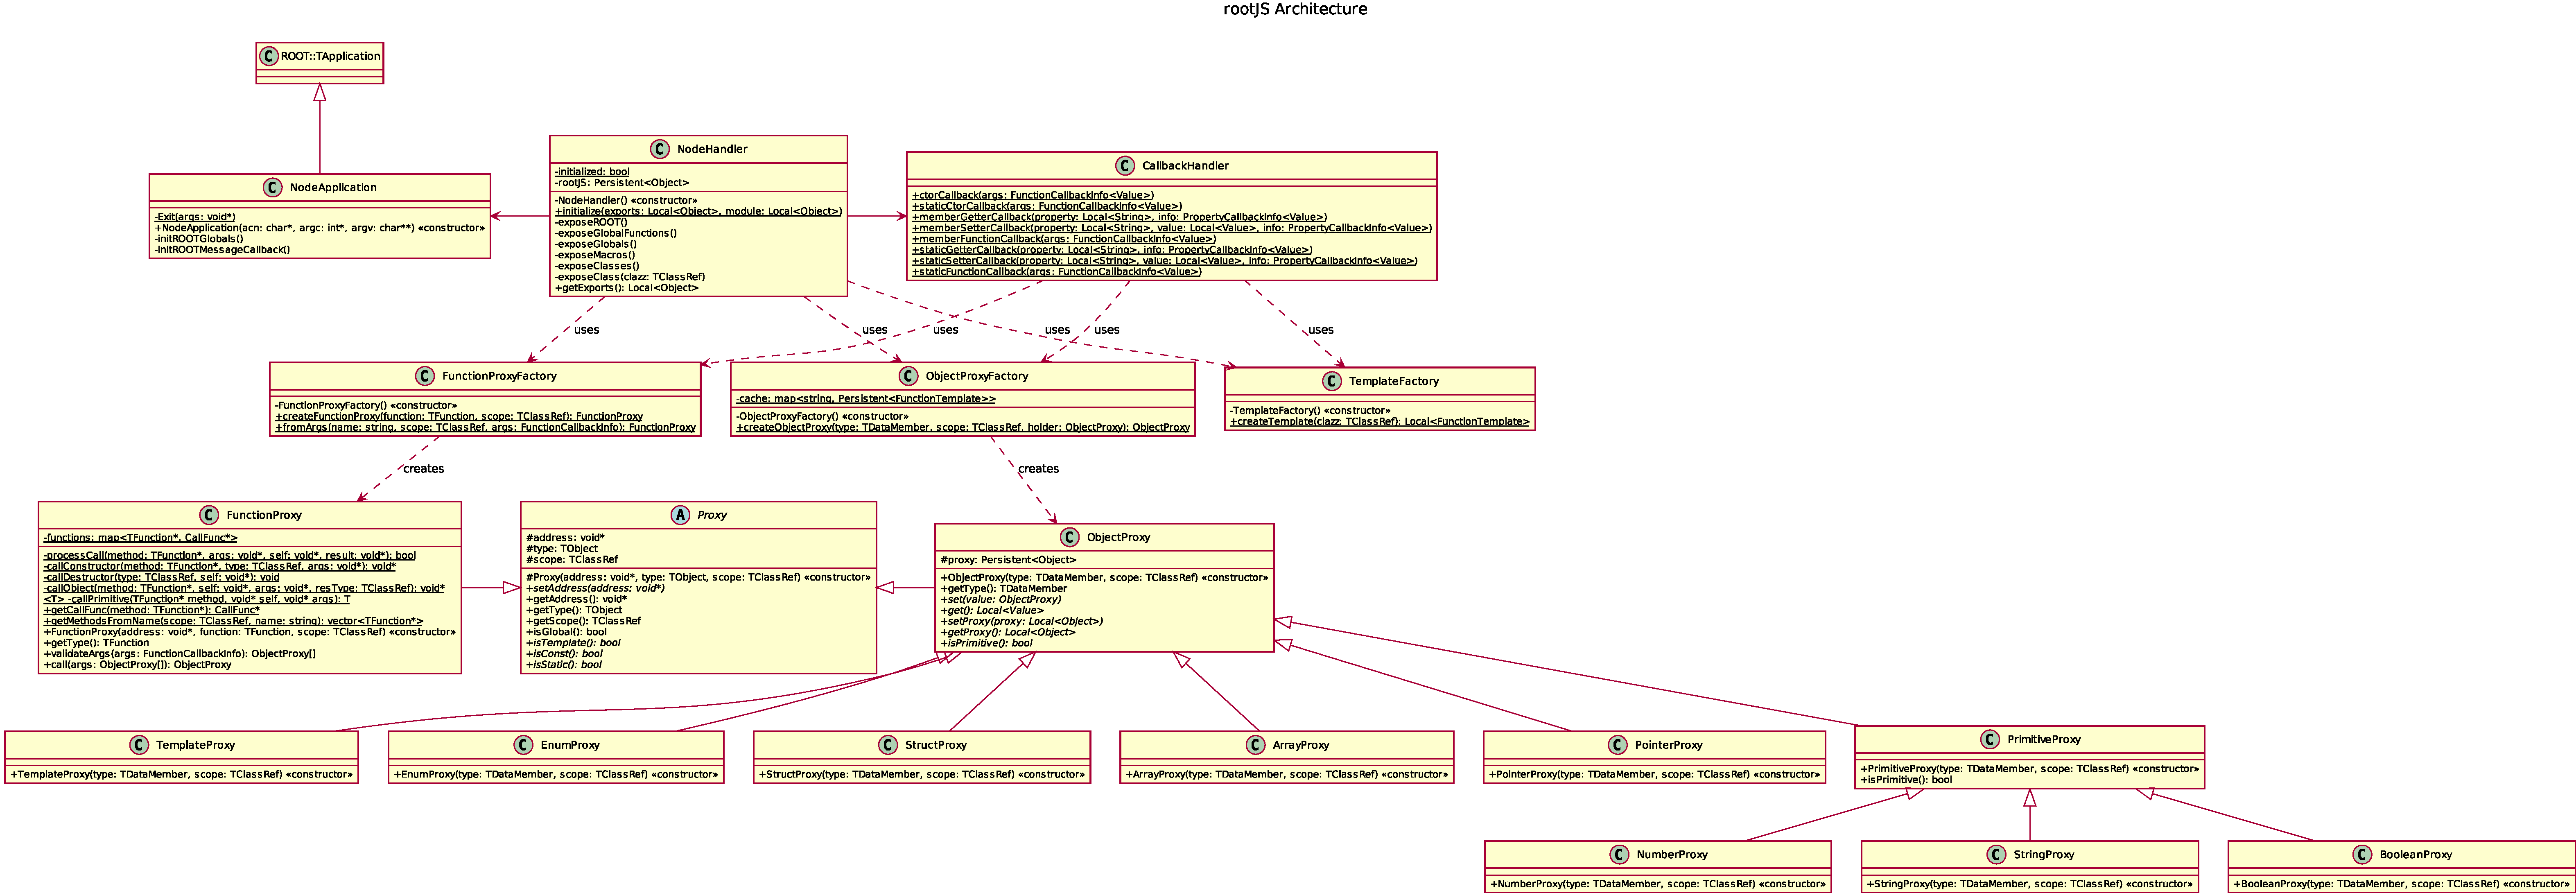
\includegraphics[keepaspectratio=true, width=7.75in, 
	angle=90]{./latex/oldResources/architecture.pdf}
	\caption{The rootJS class diagram at the conclusion of the design phase}
\end{figure}


\begin{figure}[H]
	\centering
	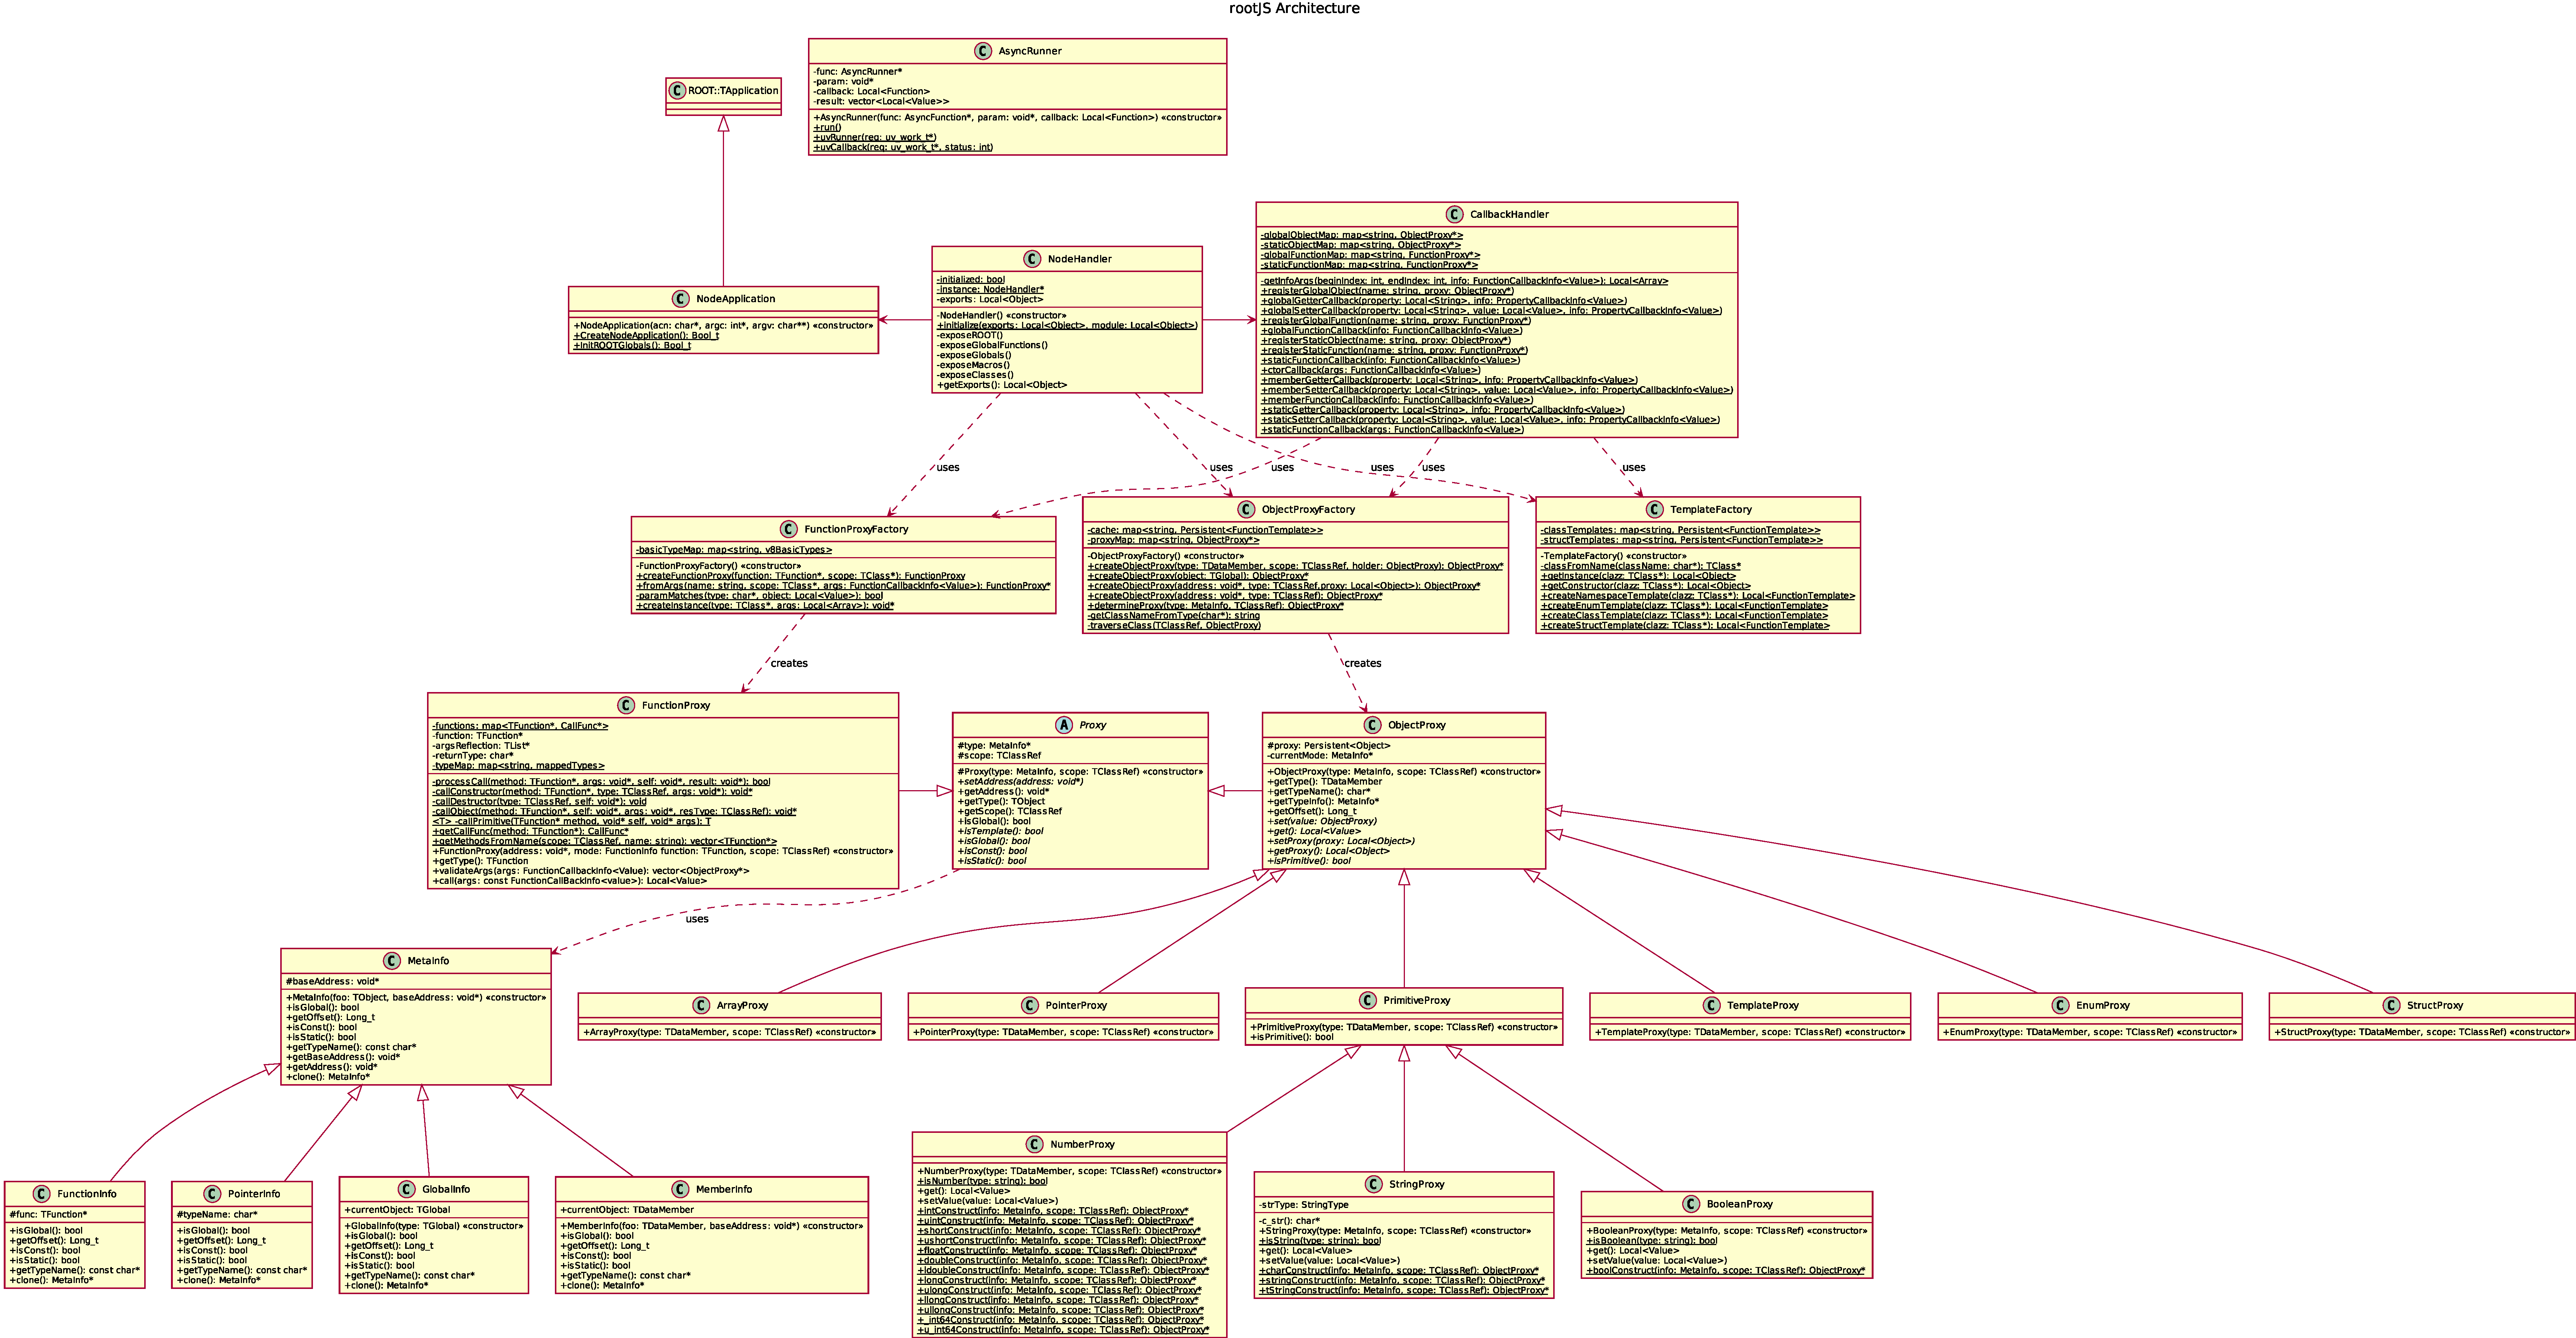
\includegraphics[keepaspectratio=true, width=9in,
	 angle=90]{./latex/resources/architecture.pdf}
	\caption{The current rootJS class diagram }
\end{figure}
\section{The Changes in the Architecture in detail}
\begin{itemize}
	\item MetaInfo
\end{itemize}
The MetaInfo class and its subclasses MemberInfo, GlobalInfo, PointerInfo and FunctionInfo were added to encapsulate the 
differences between TGlobals and TDataMembers. In the initial design, an ObjectProxy would have had to handle
both TGlobals and TDataMembers, but there subtle differences between them. One of them would be that TDataMembers 
have an offset while TGlobals do not. Therefore there was a need to create a class which contains the specific information 
of them. Later it turned out that TFunctions and pointers also require an information class. 
Now an ObjectProxy instance can only be created with the constructor if a MetaInfo class is passed as a parameter.
\begin{itemize}
	\item AsyncRunner
\end{itemize}

\begin{itemize}
	\item TemplateFactory
\end{itemize}
\begin{itemize}
	\item FunctionProxyFactory
\end{itemize}
\begin{itemize}
	\item clone() and backup()
\end{itemize}
\begin{itemize}
	\item ObjectProxyFactory
\end{itemize}
\begin{itemize}
	\item primitives construct methods
\end{itemize}



